% !TEX root = Theo_III.tex

\usepackage{tikz}
\usetikzlibrary{arrows.meta,positioning,decorations.markings,intersections,calc}


\tikzset{
legreen/.style={green!50!black},
charge color/.style={blue!50!white!70!black},
coordsystem/.style={very thin, color=#1!50},
invisiblePoint/.style={circle,inner sep=0pt,outer sep=0pt,minimum size=0pt},
point/.style={invisiblePoint,fill=black,minimum size=4pt},
arr/.style={->,>={Stealth},thin},
midarrow/.style={postaction=decorate,decoration={markings, mark=at position #1 with {\arrow{Stealth}}} },
midarrow/.default=.5,
rmidarrow/.style={postaction=decorate,decoration={markings, mark=at position #1 with {\arrowreversed{Stealth}}} },
rmidarrow/.default=.5,
distance marker/.style={|<->|,>={Stealth}},
}
\tikzstyle{every node}=[font=\footnotesize]


\newcommand{\tfigWatermolecule}{

    % water molecule
    \begin{tikzpicture}[scale=3]
        \node[circle] (H1) at ($(-90+104.45/2:1)$) {$\mathrm{H}^+$};
        \node[circle] (H2) at ($(-90-104.45/2:1)$) {$\mathrm{H}^+$};
        \node[circle] (p) at (-90:.8) {};
        \node[circle] at (0,0) [label={east,xshift=-2mm,yshift=1mm}:-] {O} 
            edge (H1) 
            edge (H2) 
            edge[arr, charge color] 
            node[midway, left] {$\vec p$} (p);
    \end{tikzpicture}
}

\newcommand{\tfigElementalQuadrupoles}{
    % elemental quadrupoles
    \begin{tikzpicture}[
        scale=1.2,
        charge/.style={point, charge color, outer sep=2mm}
    ]
    \node[charge] (Q1) at (-1,-1) [label={left}:$+q$] {};
    \node[charge] at (-1,1) [label={left}:$-q$] {} edge[arr] (Q1);
    \node[charge] (Q2) at (1,1) [label={left}:$+q$] {};
    \node[charge] at (1,-1) [label={left}:$-q$] {} edge[arr] (Q2);


    \begin{scope}[shift={(5,0)}]
        \node[charge] (Q3) at (0,1) [label={left}:$+q$] {};
        \node[charge] (Q4) at (0,-1) [label={left}:$+q$] {};
        \node[charge, inner sep=1mm] at (0,0) [label={left}:$-2q$] {} 
            edge[arr] (Q3) 
            edge[arr] (Q4);
    \end{scope}
    \end{tikzpicture}
}

\newcommand{\tfigMagnetfeldBeiLeiter}{
    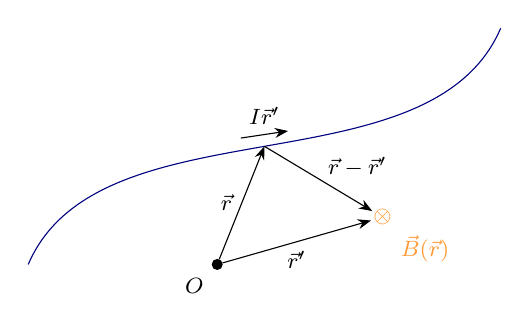
\begin{tikzpicture}[scale=3]
        \coordinate (O) at (0. 8,0);   % Koordinatenursprung
        \coordinate (A) at (1, 0.5);   % Punkt auf Leiter
        \coordinate (B) at (1.5, 0.2); % Punkt, wo Magnetfeld ausgewertet wird
        
        % Leiter (Kurve)
        \draw[color=blue!50!black] (0,0) .. controls (.3,.7) and (1.7,.3) .. (2,1);
        % Stromelement Idr
        \draw[arr] (1-0.1, 0.55-0.015) -- +(0.2, 0.03) 
            node[midway, above] {$I \diff \vec r'$}; 
            
        % Punkt, wo Magnetfeld ausgewertet wird
        \node[invisiblePoint,text=orange!80] (b point) at (B) 
            [label={south east}:\textcolor{orange!80}{$\vec B(\vec r)$}] {$\mathbf{\otimes}$};
        % Punkt auf Leiter
        \node[invisiblePoint] (conductor point) at (A) {}
            edge[arr] node[midway,auto,yshift=-1mm] {$\vec r-\vec r'$} 
            (b point);
        % Ursprung
        \node[point] (origin) at (O) [label={south west}:$O$] {} 
            edge[arr] node[midway,left] {$\vec r$} 
            (conductor point) 
            edge[arr] node[midway,below] {$\vec r'$} 
            (b point);
            
    \end{tikzpicture}
}
\newcommand{\tfigEfieldAndPotLinesAndChargeDensitityHomoChargedSphere}{
    % Field and equipotential lines of a charged sphere
    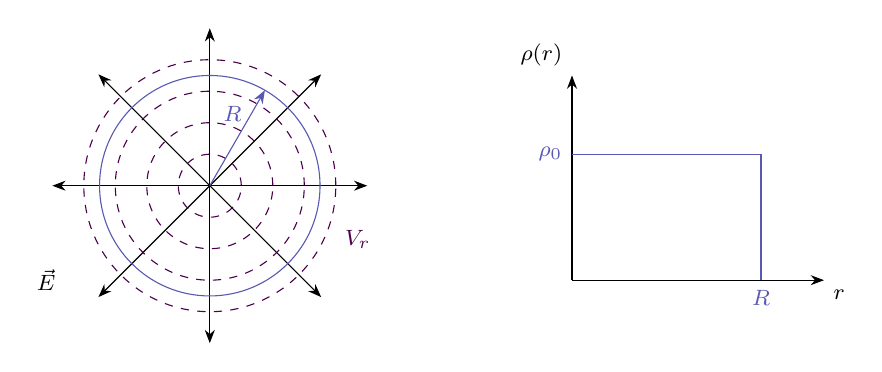
\begin{tikzpicture}[
        scale=2,
        potential color/.style={violet!60!black}
    ]
    \coordinate (O) at (0.0,0.0);

    \foreach \angle in {0,45,...,325}
        \draw[arr] (O) -- (\angle:1);
    \foreach \radius in {0,0.2,...,0.8}
        \draw[dashed,potential color] (O) circle [radius=\radius];
        
    \node[potential color] at (-20:1) {$V_r$};
    \node at (-150:1.2) {$\vec E$};

    \draw[charge color] (O) circle [radius=.7];
    \draw[arr, charge color] (O) -- (60:0.7) node[near end, left] {$R$};

    \begin{scope}[shift={(2.3,-.6)}]
        \coordinate (A) at (1.2, 0.8);
        
        \draw[arr] (0,0) -- (0, 1.3) 
            node[at end, anchor=south east] {$\rho(r)$};
        \draw[arr] (0,0) -- (1.6, 0) 
            node[at end, anchor=north west] {$r$};
        \draw[charge color] let \p1 = (A) in
            (0, \y1) -- (A) 
            node[at start, left] {$\rho_0$}
            -- (\x1, 0)
            node[charge color, below] {$R$};
    \end{scope}
    \end{tikzpicture}
}
\newcommand{\tfigEfieldAndPotentialHomoChargedSphere}{
    % field and potential function for sphere
    \begin{tikzpicture}[scale=3]
        \coordinate (A) at (0.8, 0.8);
        
        % electric field
        \draw[arr] (0,0) -- +(0, 1.1) 
            node[at end, anchor=south east] {$E(r)$};
        \draw[arr] (0,0) -- +(1.8, 0) 
            node[at end, anchor=north west] {$r$};
            
        \draw[charge color,yscale=.2] 
            let \n1={0.5},\n2={1.7} in
            plot[domain=0:\n1] (\x,\x/\n1^3) 
            node[above left] at (\n1/2,\n1/2/\n1^3) {$\propto r$} 
            plot[domain=\n1:\n2] (\x,1/\x^2) 
            let \n4={.5*\n2-.5*\n1+\n1} in % x value of middle point of second graph 
            node[above] at (\n4,1/\n4^2) {$\propto\frac{1}{r^2}$};
        \draw[dashed, very thin] (0.5,.8) -- +(0,-.8) 
            node[below] {$R$};
            
        % potential
        \begin{scope}[shift={(2.5,0)}]
            \draw[arr] (0,0) -- +(0, 1.1) 
                node[at end, anchor=south east] {$\phi(r)$};
            \draw[arr] (0,0) -- +(1.8, 0) 
                node[at end, anchor=north west] {$r$};
            \draw[charge color,yscale=.3] 
                let \n1={0.5},\n2={1.7} in 
                plot[domain=0:\n1] (\x,3/\n1/2 -\x^2/\n1^3/2)
                node[right, xshift=-25,yshift=25] {$\propto \frac3{2R}-\frac{r^2}{2R^3}$}
                plot[domain=\n1:\n2] (\x,1/\x)
                let \n4={.5*\n2-.5*\n1+\n1} in % x value of middle point of second graph 
                node[above] at (\n4,1/\n4) {$\propto\frac{1}{r}$};
                
            \draw[dashed, very thin] (0.5,1/1.7) -- +(0,-1/1.7) 
                node[below] {$R$};
        \end{scope}
    \end{tikzpicture}
}

\newcommand{\tfighysterese}{
    \begin{tikzpicture}[scale=2]

        \coordinate (saturation) at (1,1);
        \coordinate (inv saturation) at (-1,-1);

        % Axis
        \draw[name path=xaxis,arr] (-1.4,0) -- (1.4,0) node[anchor=north west] {$H$};
        \draw[name path=yaxis,arr] (0,-1.4) -- (0,1.4) node[anchor=south east] {$B$};

        % Curve (1) (magnetize)
        \draw[midarrow,dashed,color=blue!50!black]
        (0,0) .. controls (0.3,.2) and (0.1,1) .. (saturation)
        node[midway,right,xshift=-1.5mm,yshift=-2mm] {(1)};
        % Curve (2)  (change field to negative)
        \draw[name path=dcurve, midarrow,color=blue!50!green]
        (saturation) .. controls (-0.8,1) and (-0.1,-1) .. (inv saturation)
        node[near end,left] {(2)};
        % Curve (2)  (change field to positive)
        \draw[midarrow,color=blue!60!white!70!black]
        (inv saturation) .. controls (0.8,-1) and (0.1,1) .. (saturation)
        node[near start,right,xshift=1mm,yshift=1mm] {(3)};
        % Coordinates of Saturation
        \draw[dashed] (saturation) -- (1,0)
        node[below] {$H_\mathrm{S}$};
        \draw[dashed] (saturation) -- (0,1)
        node[left] {$B_\mathrm{S}$};

        % Remanence and coercitive field
        \path[name intersections={of=yaxis and dcurve, by=remanenz}];
        \path[name intersections={of=xaxis and dcurve, by=coercitive}];
        \draw ($(remanenz)+(1pt,0)$) -- ($(remanenz)-(1pt,0)$)
        node[left] {$B_\mathrm{R}$};
        \draw ($(coercitive)+(0,1pt)$) -- ($(coercitive)-(0,1pt)$)
        node[anchor=north west,xshift=-2mm] {$H_\mathrm{C}$};

    \end{tikzpicture}
}

\newcommand{\tfigMagneticRefraction}{
    \begin{tikzpicture}[
            scale=2,
            incolor/.style = {red!50!black},
            outcolor/.style = {blue!50!black}
        ]
        \coordinate (Start) at (-2,-0.5);
        \coordinate (StartFoot) at ($(Start) + (0,.2)$);
        \coordinate (Middle) at (0,-0.3);
        \coordinate (End) at (0.4,0.2);
        \coordinate (EndFoot) at (0,0.2);

        \draw (0,1) -- (0,-.6);
        \node[circle] at (-1,.9) {$\mu_1$};
        \node[circle] at (.5,.9) {$\mu_2\gg\mu_1$};

        \draw[arr, incolor] (Start) -- (Middle)
        node[midway, below] {$\vec H^{(1)}$};
        \draw[arr, outcolor] (Middle) -- (End)
        node[midway, right] {$\vec H^{(2)}$};
        \draw[dashed, incolor] (Start) -- (StartFoot)
        node[midway,left] {$H_\parallel^{(1)}$}
        -- (Middle) node[midway, above] {$H_\perp^{(1)}$};
        \draw[dashed, outcolor] (EndFoot)
        -- (End) node[midway, above] {$H_\perp^{(2)}$};
    \end{tikzpicture}
}


\newcommand{\tfigConductorLoopWithRefPoint}{
    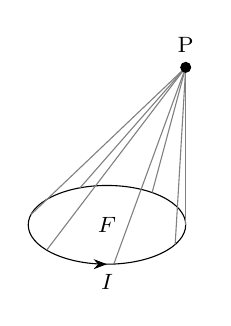
\begin{tikzpicture}[scale=1]
        \coordinate (O) at (0,0);
        \coordinate (P) at (1,2);
        \draw[midarrow=.75] (O) ellipse [x radius=1, y radius=.5]
        node[] {$F$};
        \node[below] at (0,-.5) {$I$};
        \foreach \angle in{0, 55, ..., 360}
        \draw[gray] ($cos(\angle)*(1,0)+sin(\angle)*(0,.5)$) -- (P);
        \node[point] at (P) [label=P]{};
    \end{tikzpicture}
}

% \newcommand{\tfigMagneticFeldHomogenousBall}{
%     \begin{tikzpicture}[
%             scale=.7,
%             mcolor/.style=legreen,
%             pics/graph/.style={background code={
%                             \coordinate (O) at (0,0);
%                             \coordinate (P) at (1,2);
%                             \draw (O) circle [radius=1];
%                             \foreach \vzx in {1,-1}{
%                                     \draw[midarrow] (\vzx*0.5,0.866) ..
%                                     controls ($1.2*(\vzx*0.5,0.866)$)
%                                     and (\vzx*1.2, 2.4) .. (\vzx*2.5,3);
%                                     \draw[midarrow] (\vzx*2.5,-3) ..
%                                     controls (\vzx*1.2,-2.4)
%                                     and ($1.2*(\vzx*0.5,-0.866)$) .. (\vzx*0.5,-0.866);
%                                     \draw[midarrow=.51] (\vzx*0.866,0.5)
%                                     .. controls +($.8*(\vzx*0.866,0.5)$)
%                                     and (\vzx*3,1)
%                                     .. (\vzx*3,0)
%                                     .. controls (\vzx*3,-1) and ($1.6*(\vzx*0.866,-0.5)$)
%                                     .. (\vzx*0.866,-0.5) ;
%                                     \draw[arr] (\vzx*0.866,#1*-0.4) -- (\vzx*0.866,#1*0.4);
%                                     \draw[arr] (\vzx*0.5,#1*-0.8) -- (\vzx*0.5,#1*0.8);
%                                     \draw[arr, mcolor] (\vzx*0.7,-0.4) -- +(0,0.8);
%                                     \draw[arr, mcolor] (\vzx*0.25,-0.4) -- +(0,0.8);
%                                 }
%                             \draw[midarrow=.6] (0,1) -- (0,3.2);
%                             \draw[midarrow=.4] (0,-3.2) -- (0,-1);
%                             \draw[arr] (0,#1*-.9) -- (0,#1*0.9);
%                         }}
%         ]

%         %\pic=1 at (0,0) [transform shape]{graph};
%         %\pic at (7,0) [transform shape]{graph};

%         \draw (0,0) pic[transform shape] {graph=1} node[outer sep=70,above] {$\vec B$-Feld};
%         \draw (7,0) pic[transform shape] {graph=-1} node[outer sep=70,above] {$\vec H$-Feld};
%         \node[mcolor] at (-1.5,0) {$\vec M$};
%         \node[mcolor] at (-1.5+7,0) {$\vec M$};

%     \end{tikzpicture}
% }


\newcommand{\tfigCoil}{
    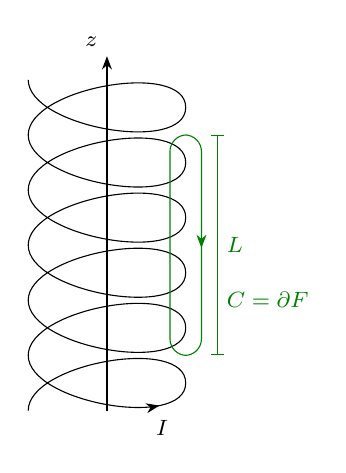
\begin{tikzpicture}[scale=1]
        \draw[arr] (0,0) -- (0,4.5)
        node[anchor=south east] {$z$};

        \draw[rmidarrow=.10] (-1,0)
        \foreach \a in {1,...,6}{
                .. controls +(0,.6) and +(0,.6)
                .. +(2,.35)
                .. controls +(0,-.6) and +(0,-.6)
                .. ++(0,.7)
            };
        \node[anchor=north west] at (.5,0) {$I$};
        \draw[legreen, rounded corners=6pt, midarrow=.7]
        (.8,.7) rectangle (1.2,3.5);
        \draw[legreen, |-|] (1.4,.7) -- +(0,2.8)
        node[midway, right] {$L$}
        node[near start, right] {$C=\partial F$};
    \end{tikzpicture}
}

\newcommand{\tfigInductionA}{
    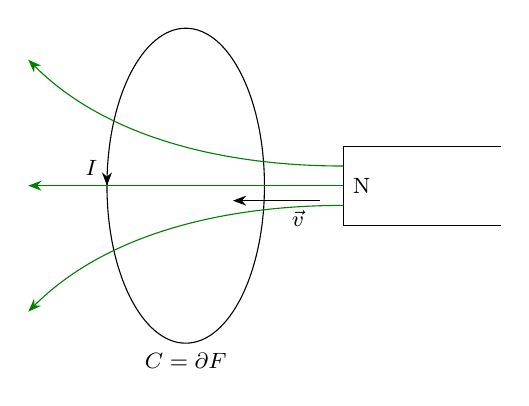
\begin{tikzpicture}[scale=1]
        \draw[midarrow=.5] (0,0)
        ellipse[x radius=1, y radius=2];

        \draw (4, -.5) -- ++(-2,0)
        -- ++(0,1) node[midway, right] {N}
        -- +(2,0);
        \draw[arr] (1.7,-.19) -- ++(-1.1,0) node[near start, below] {$\vec v$};
        \node[below] at (0,-2) {$C=\partial F$};
        \node[anchor=south east] at (-1,0) {$I$};
        \draw[legreen,arr] (2,0.25) .. controls +(-1.5,0) and +(1,-1) .. (-2,1.6);
        \draw[legreen,arr] (2,-0.25) .. controls +(-1.5,0) and +(1,1) .. (-2,-1.6);
        \draw[legreen,arr] (2,0) -- (-2,0);
    \end{tikzpicture}
}

\newcommand{\tfigInductionB}{
    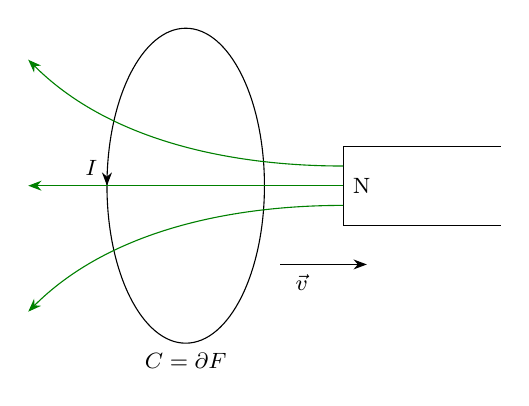
\begin{tikzpicture}[scale=1]
        \draw[midarrow=.5] (0,0)
        ellipse[x radius=1, y radius=2];

        \draw (4, -.5) -- ++(-2,0)
        -- ++(0,1) node[midway, right] {N}
        -- +(2,0);
        \draw[arr] (1.2,-1) -- ++(1.1,0) node[near start, below] {$\vec v$};
        \node[below] at (0,-2) {$C=\partial F$};
        \node[anchor=south east] at (-1,0) {$I$};
        \draw[legreen,arr] (2,0.25) .. controls +(-1.5,0) and +(1,-1) .. (-2,1.6);
        \draw[legreen,arr] (2,-0.25) .. controls +(-1.5,0) and +(1,1) .. (-2,-1.6);
        \draw[legreen,arr] (2,0) -- (-2,0);
    \end{tikzpicture}
}


\newcommand{\tfigcylindricalConductorAndCoil}{
    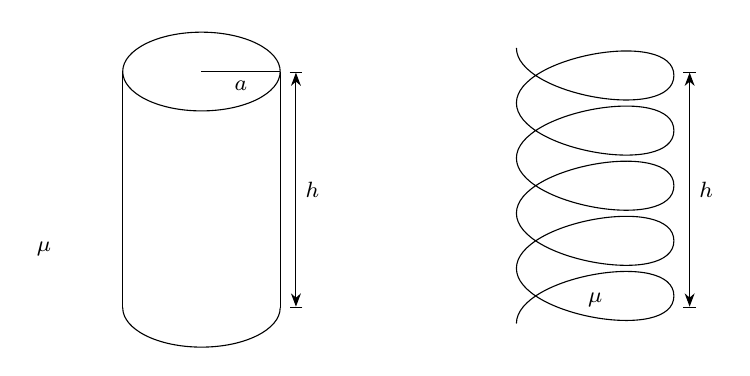
\begin{tikzpicture}[scale=1]
        \coordinate (bottom) at (0,0);
        \coordinate (top) at (0,3);
        \coordinate (offset) at (1,0);

        % cylindrical conductor
        \draw (top)
        ellipse[x radius=1, y radius=.5];
        \draw
        ($(bottom) + (offset)$)
        arc[start angle=0, end angle=-180, x radius=1, y radius=.5];
        \draw
        ($(bottom) + (offset)$) -- ($(top) + (offset)$)
        ($(bottom) - (offset)$) -- ($(top) - (offset)$);
        \draw
        (top) -- ($(top) + (offset)$)
        node[midway, below] {$a$};
        \draw[distance marker]
        ($(bottom) + (offset) + (.2, 0)$) -- +(top)
        node[midway, right] {$h$};
        \node at ($(bottom) + (-2,.75)$) {$\mu$};
        % coil
        \begin{scope}[shift={(4,0)}]
            \draw (0,-.2)
            \foreach \a in {1,...,5}{
                .. controls +(0,.6) and +(0,.6)
                .. +(2,.35)
                .. controls +(0,-.6) and +(0,-.6)
                .. ++(0,.7)
            };
            \node at (1,0.1) {$\mu$};
            \draw[distance marker]
                (2.2, 0) -- +(0,3)
                node[midway, right] {$h$};
        \end{scope}
    \end{tikzpicture}
}


\newcommand{\tfigTwoInductors}{
    \begin{tikzpicture}[scale=1]
        \draw[rotate=20, midarrow=0.75]
        (0,0) ellipse [x radius=1, y radius=.5]
        node {$C_1$}
        node[xshift=13, yshift=-20] {$I_1$};
        \draw[rotate=-40, midarrow=0.75]
        (3,0) ellipse [x radius=1, y radius=.5]
        node {$C_2$}
        node[xshift=-13, yshift=-20] {$I_2$};
        \node at (0,-2) {$\mu$};
        \node at (3,0) {$\ldots$};
    \end{tikzpicture}
}

\newcommand{\tfigGrenzflaecheMagnetic}{
    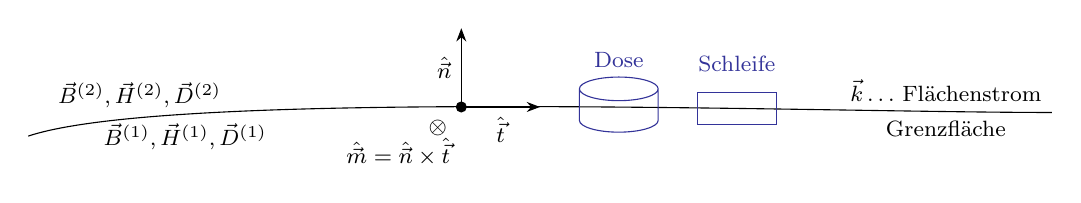
\begin{tikzpicture}[
            scale=1,
            dosenfarbe/.style={blue!50!black!80!white}
        ]
        \draw
        (0,0) .. controls (1.8,.6) and +(-3,0) .. (13,.3)
        node[pos=.17, above] {$\vec B^{(2)},\vec H^{(2)},\vec D^{(2)}$}
        node[pos=.22, below] {$\vec B^{(1)},\vec H^{(1)},\vec D^{(1)}$}
        node[very near end, above] {$\vec k\ldots$ Flächenstrom}
        node[very near end, below] {Grenzfläche};

        \coordinate (P) at (5.5, .37);

        \node[point] at (P) {};
        \draw[arr]
        (P) -- +(0:1)
        node[midway, below] {$\hat{\vec t}$};
        \draw[arr]
        (P) -- +(90:1)
        node[midway, left] {$\hat{\vec n}$};

        \node at (5.2,.1) {$\otimes$}
        node at(4.7,-.2) {$\hat{\vec m}=\hat{\vec n}\times\hat{\vec t}$};

        \draw [dosenfarbe]
        (7,.6) -- +(0,-.4)
        arc[start angle=-180, end angle=0,x radius=.5, y radius=.15]
        -- +(0,.4)
        arc[start angle=0, end angle=180,x radius=.5, y radius=.15]
        node[midway, above] {Dose}
        arc[start angle=-180, end angle=0,x radius=.5, y radius=.15];
        \draw[dosenfarbe]
        (8.5,.55) rectangle +(1,-0.4) node[midway,above,yshift=10] {Schleife};
    \end{tikzpicture}
}


\newcommand{\tfigBewegungDurchLichtaetherA}{
    \begin{tikzpicture}[scale=3]
        \begin{scope}
            \draw[arr] (0,0) -- (0,1)
                node[anchor=south east] {$\vec e_2$};
            \draw[arr] (0,0) -- (1,0)
                node[anchor=north west] {$\vec e_1$};
            \node at (.5,.5) {Äther};
        \end{scope}
        \begin{scope}[shift={(2cm,0)}]
            \draw[arr] (0,0) -- (0,1)
                node[anchor=south east] {$\vec e_2$};
            \draw[arr] (0,0) -- (1,0)
                node[anchor=north west] {$\vec e_1$};
            \node at (.5,.5) {Erde};

            \draw[arr] (.2,.2) -- +(.6,0) node[anchor=west] {$\vec v=v \vec e_1$};            
        \end{scope}
    \end{tikzpicture}
}

\newcommand{\tfigBewegungDurchLichtaetherB}{
    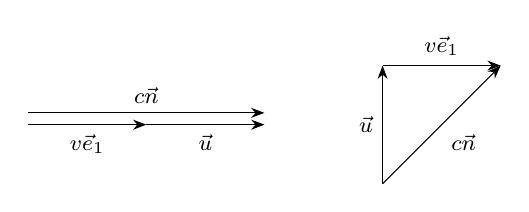
\begin{tikzpicture}[scale=1.5]
        \begin{scope}
            \draw[arr] (0,0) -- +(1,0)
                node[midway, below] {$v\vec e_1$};
            \draw[arr] (1,0) -- +(1,0)
                node[midway, below] {$\vec u$};
            \draw[arr] (0,.1) -- +(2,0)
                node[midway, above] {$c \vec n$};
        \end{scope}

        \begin{scope}[shift={(3cm,-0.5cm)}]
            \draw[arr] (0,0) -- (0,1)
                node[midway, left] {$\vec u$};
            \draw[arr] (0,1) -- +(1,0)
                node[midway, above] {$v\vec e_1$};
            \draw[arr] (0,0) -- +(1,1)
                node[midway, anchor=north west] {$c\vec n$};

        \end{scope}
    \end{tikzpicture}
}

\newcommand{\tfigMichelsonInterferometer}{
    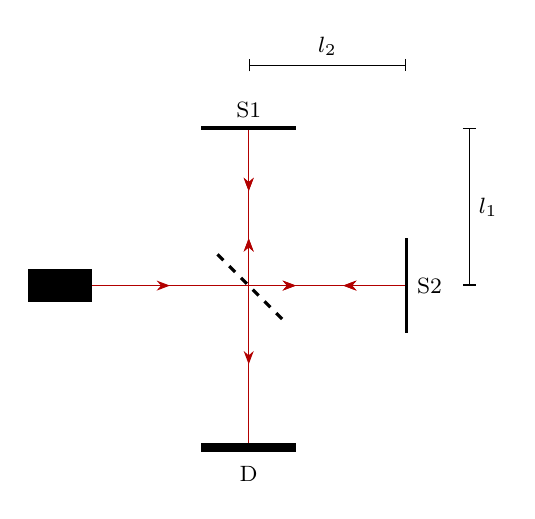
\begin{tikzpicture}[
            scale=2,
            light/.style={red!70!black}
        ]
        \coordinate (ST) at (0,0);
        \coordinate (L) at (-1,0);
        \coordinate (S1) at (0,1);
        \coordinate (S2) at (1,0);
        \coordinate (D) at (0,-1);

        \draw[midarrow, light] (L) -- (ST);
        \draw[midarrow=.3, rmidarrow=.6, light] (ST) -- (S1);
        \draw[midarrow=.3, rmidarrow=.6, light] (ST) -- (S2);
        \draw[midarrow, light] (ST) -- (D);

        \draw[dashed, very thick] ($(ST) + (-45:.3)$) -- ($(ST) - (-45:.3)$);
        \draw[very thick] ($(S1) + (.3,0)$) -- ($(S1) - (.3,0)$)
            node[midway, above] {S1};
        \draw[very thick] ($(S2) + (0,.3)$) -- ($(S2) - (0,.3)$)
            node[midway, right] {S2};
        
        \draw[fill=black] ($(L) - (.4, .1)$) rectangle ($(L) + (0, .1)$);
        \draw[fill=black] ($(D) - (.3, .05)$) rectangle ($(D) + (.3, 0)$)
            node[midway, below, yshift=-1.2mm] {D};

        \draw[|-|] let \p1 = (S1), \p2 = (S2) in 
            (\x2 + .4cm,\y1) -- (\x2 +.4cm, 0) 
            node[midway, right] {$l_1$};
        \draw[|-|] let \p1 = (S1), \p2 = (S2) in 
            (0,\y1 +.4cm) -- (\x2,\y1 +.4cm) 
            node[midway, above] {$l_2$};
    \end{tikzpicture}
}